\documentclass[12pt]{article}
\renewcommand{\baselinestretch}{1.4}
\usepackage{graphicx}

\usepackage[light,math]{iwona}
\usepackage[T1]{fontenc}


\begin{document}

\tableofcontents

\section{Foreword}
This is my English handout about Machine Learning and Deep Learning, and please excuse me from all readers for the sake of my some bad English Terminology in whole of this handout or "article". Why i choice English language for this handout? Because i will push this handout in universe repo such as GitHub or Google scholar for help someone that want learn ML and DL and etc.

\newpage

\section{What is ML}

\LARGE What is Machine Learning?\\
\small Machine Learning is a method of data analysis that automates analytical model building.\\
using algorithms that iteratively learn from data, machine learning allows computers to find hidden insights without begin explicitly programmed where to look, What is this mean? that's mean if you want create an program in Python that can tell you what you input in program, for example can say output is Blue or Red color, you maybe use some statement(if, else, elif), in ML we don't use from that!

\subsection{What is it used for?}
Machine Learning is used in a with variety of topics and use cases every things from fraud Detection to web search results to credit scoring. Or maybe you're traveling abroad and ease your credit cart and you get a call indication a possible fraud on your credit card. That's also ML attempting to detect fraudulent use cases. Then there is things like \textbf{recommendation} engines, so if you're shopping on somethings like Amazon or Digikala.com or even viewing some online streaming video service and it's recommending new videos or new movies or new TV shows to you, ML is used for that as well and things like e-mail spam filtering so the e-mails that actually go into your span folder that's using natural language processing
\footnote{NLP}to figure out what is the actual spam email and then things like pattern and image recognition. \\

Now there's certain use cases where the only possible approach is to use Deep Learning.    


\section{What are Neural Networks}
For the basics Neural Networks are way of modeling biological and you're on systems mathematically and these networks can then be used to solve tasks that many other types of algorithms can't. 
So for example that image classification it's really hard for other ML algorithms to perform well on things like image classification, and this is the kind of task where neural networks perform very well. 
So \textbf{deep learning} simply refers to neural networks with more than one hidden layer. \\

There are different types of machine learning "tasks" we will focus on during the next section.

As a quick review what is say In final note:\\
\textbf{Machine Learning}: Those are just a general terms for those automated analytical models.\\
\textbf{Neural Networks}: is actually a specific type of machine learning architecture or algorithm that specifically modeled after biological neurons.\\
\textbf{Deep Learning}: is really just a neural network with more than one hidden layer.\\ 
And we will discuss, what that means and what a hidden layer actually is in the Artificial Neural Networks in next section.\\

\section{Different between Supervised and Unsupervised Learning}

\subsection{Supervised Learning}
supervised learning algorithms are trained using labeled example and that's a keyword label such as an input where the desired output is known, that means within your dataset you're going to have some historical feature with historical labels.
So you already have that information such as segment of text could have a category label, so you take a bunch of previous e-mails and someone has already gone by and classified then using the correct label, they read the e-mail and classified it as span versus legitimate or we have a bunch of movies reviews and someone has already gone and labeled movie reviews either positive to the movie or negative to the movie and then the idea would be for future text information such as a future e-mail using the historical label data the network or Machine Learning algorithm could learn off the historical data in order to predict for new data whether it belongs i the span category or legitimate category or in the   positive category or negative category for these movie reviews so the way this works is for \textbf{neural networks} the networks and receive a set of input data along with the corresponding correct outputs and then algorithm or  network will learn by comparing its actual output with correct outputs to find errors and then it will modify the model accordingly such as adjusting the weights and biased value in the network.\\
Supervised learning is commonly used in applications where historical data predicts likely future event.\\

\subsubsection{Machine Learning Process}
The first thing to do is actually \textbf{get data} and depends on what \textbf{domain} you're working in where this data actually comes from. This can come from your customers or can come from collecting things into a database online or maybe it's physical data and it comes from sensors etc...\\

So At some point the data has to actually be acquired one we actually acquire the data then we need to clean and format the data so that our neural network can actually process it and often we will do this using a library called \textbf{PANDAS} the we split the data into \textbf{Training data} and \textbf{test data} and we talk more about this in next section. 

with Training data we build our model or network, and then run that test data through the model and compare the model's prediction to the actual correct label that the test data ahead because remember we actually know the correct label for that test data. 
You can run that test data feature through the model get our models predictions and compare it to the right answer and then we can evaluate the model and then maybe you want to go back based off that performance and adjust the model parameters maybe add more layers or more neurons to try to get a better fit onto that test data.

And once we're satisfied of this we can then deploy the model to the real world!


\textbf{some note is attention: }\\

What we just showed is a simplified approach to supervised learning, it contains an issue!

Is it fair to use our single split of the data to evaluate our models performance?

After all, we were given the chance to update the model parameters again and again!

\large To fix this issue specially in neural networks and deep learning, data is often split into \textbf{3 sets}:
\begin{itemize}
	\item
	\textbf{Training Data:}\\
	Used to train model parameters.
	
	\item 
	\textbf{Validation Data:}\\
	Used to determine what model hyperparameters to adjust, and related to accuracy of your model base on your parameters!
	
	\item
	\textbf{Test Data:}\\
	Used to get some final performance metric.
	
\end{itemize}

\section{Overfitting}

\begin{itemize}
	\item
	Overfitting 
	The model fits too much to the noise from the data.\\
	This often results in \textbf{low error on training set sut high error on test/validation sets}.
	
	So let's actually take a look at what overfitting would look like for the example case of really simple dataset where you just have one feature X and you're trying to predict Y. 
	\begin{figure}[htbp]
	\centerline{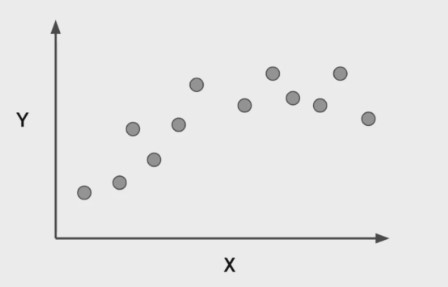
\includegraphics[scale=.5]{img/overfitting1.jpg}}
\end{figure}
	So here we have a bunch of training points and so there's some single feature X and at the end of the day we want to build out a model that can predict Y.
	
	 so a good model would try to fit the general trend pf the actual data set here so we can see it appears that there's some sort of positive slope and it looks like it levels off later on!
\begin{figure}[htbp]
\centerline{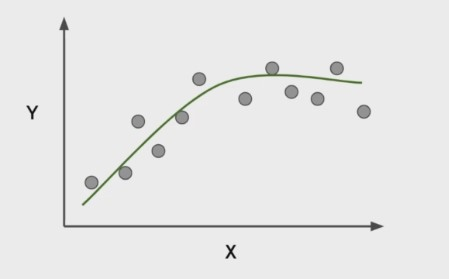
\includegraphics[scale=.5]{img/overfittingGoodModel.jpg}}
\end{figure}
 
	So what would happen if the model overfit to this training data, when you actually overfitting what's going to happen, you're actually going to fit too much to the noise of the data.
	\begin{figure}[htbp]
\centerline{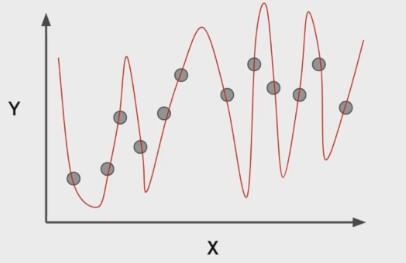
\includegraphics[scale=.5]{img/overfittingnoise.jpg}}
\end{figure}

	So here we have what appears to be a really bad model, but keep in mind that this model is technically hitting every single one of those training point. So your error here is actually going to be extremely low, and in this specific example your error is actually zero, because your model is accounting for every point in the every training set. So your error just on the training set is actually really low when you're overfitting. That's why it can be really deceptive and that's why we also need the validation and test sets in order to understand whether or not we're overfitting because just the training data alone won't tell us that information. 
	
	So, what happens when you're overfitting is your're fitting too much to the noise of the data here, if you were to get a new point and this would be a test or validation point if you're overfitting, that means you're getting low error on the training set, but when you get a new test so that the model hasn't seen before you're going to get a much larger error of your model.
		\begin{figure}[htbp]
\centerline{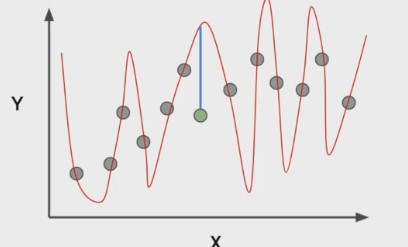
\includegraphics[scale=.5]{img/overfittingLargerError.jpg}}
\end{figure}



	
	
\end{itemize}



\section{Evaluate Performance}








\end{document}